\documentclass[11pt, a4paper, titlepage]{jsarticle} %文章クラス設定
                                                    %titlepageなくしたら,タイトルぺーぎが消えます.
\usepackage[dvipdfmx]{graphicx} %図表
\usepackage{listings} %ソースコード記載
\usepackage{amsmath, amssymb} %数式記号
\usepackage{amsthm} %定理、補題等の記述
\usepackage{bbm} %いらないかも
\usepackage{array} %数式モードで表を作成
\usepackage{siunitx} %SI単位系
\usepackage{algorithmic}
\usepackage{algorithm} %模擬コード記述
\usepackage{ascmac} %定理とかを囲う四角いやつ

%定理とかを全部,英語から日本語に変換.
\newtheorem{thm}{定理}
\newtheorem{lem}{補題}
\newtheorem{asm}{前提}
\newtheorem{rmk}{注意}
\newtheorem*{prb}{問題設定}

%証明だけ,ちょっとめんどくさかった.
\renewcommand{\proofname}{証明}
\newcommand{\argmin}{\mathop{\rm arg~min}\limits}

\makeatletter % use at mark
\renewenvironment{proof}[1][\proofname]{\par
	\pushQED{\qed}%
	\normalfont \topsep6\p@\@plus6\p@\relax
	\trivlist
	\item[\hskip\labelsep
	\itshape
	{\bf\underline{#1}}]\ignorespaces
	% {\bf\underline{#1}\@addpunct{.}}]\ignorespaces % ピリオドあり
}{%
	\popQED\endtrivlist\@endpefalse
}

%以下,タイトルを設定
\title{write title}
\author{write author name}
\date{20**/**/**}

%この下から,文章本体
\begin{document}
\maketitle
\section{First hogehoge}
ほう,hogehogeですか.
\subsection{fugafuga1}
fugafugaですね.
\subsubsection{piyo}
hogehogeって,fugafugaなpiyoなんですよね.
\subsubsection{piyopiyo}
それは,hogehogeはfugafugaでpiyopiyoだからです.
\subsection{fugafuga2}
更にfugafugaです.
\section{Second hogehoge}
第二世代のhogehogeです.方程式でも書いてみますか.
\begin{align}
    \label{hogefugapiyo1}
    hoge \triangleq \frac{fuga}{piyo}
\end{align}
この関係式\ref{hogefugapiyo1}については,以下の図に示す.

\begin{figure}[htb]
    \centerline{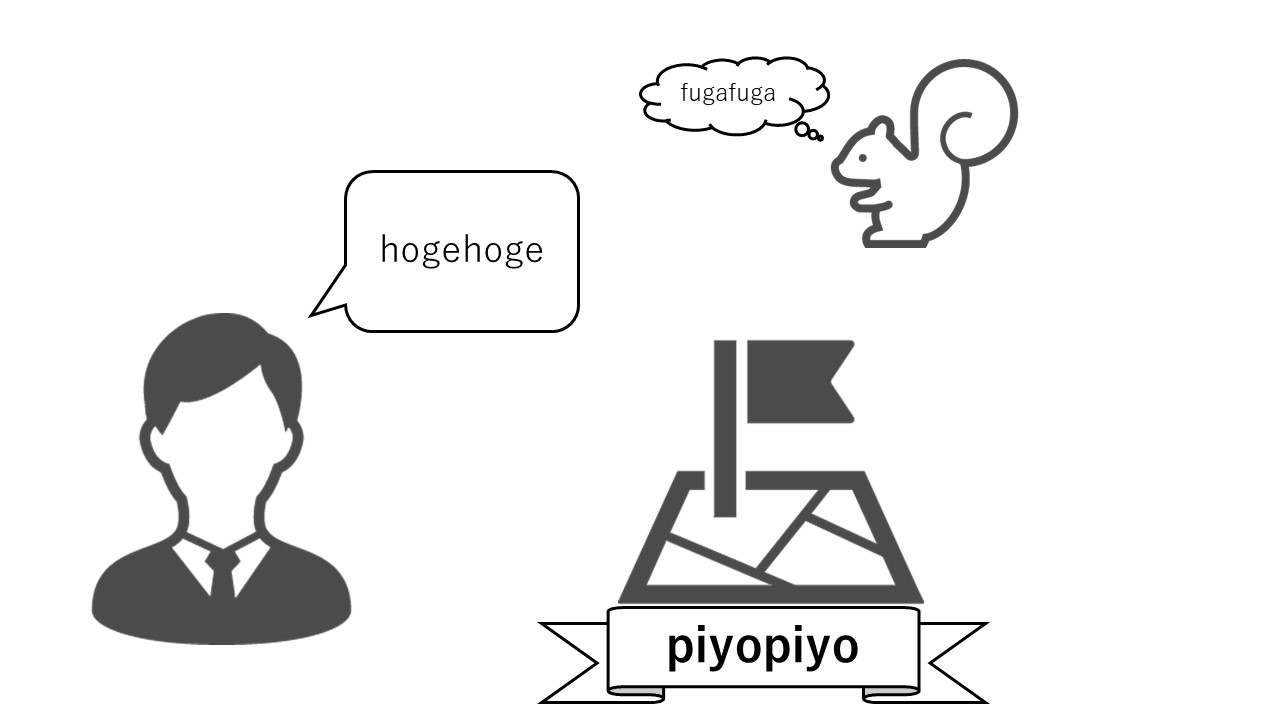
\includegraphics[scale=0.3, clip]{hogefugapiyo.jpg}}
    \caption{関係図}
    \label{hogefugapiyo2}
    \end{figure}
\end{document}